\subsubsection{Record Layout}
Each record (commonly called tuple) contains a header (which in turn contains validity flags for deletion,
visibility information for concurrency control, bit maps for null values and more), and the non-null attributes, or pointer to those attributes.

Relational engines do not have to store the schema for the tuple inside of it because that is set globally for the entire table.

Schema-less systems however have to store that information because it can differ for each record.


\paragraph{Optimizations}
\begin{wrapfigure}{l}{0.35\textwidth}
    \begin{center}
        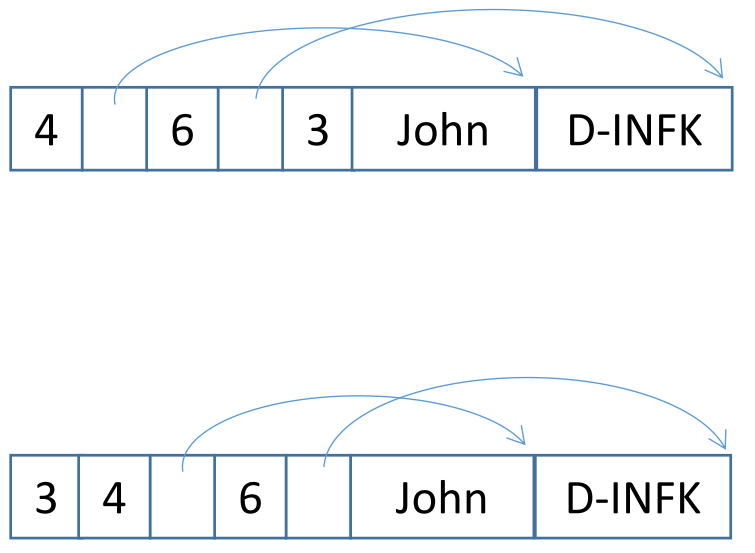
\includegraphics[width=0.3\columnwidth]{assets/db-system-record-ordering.png}
    \end{center}
    \caption{Record layouts in memory
        (Figure from Lecture 09, Slide 19)}
\end{wrapfigure}
It is crucial to store the data in a way that allows quick accesses and updates.

Each variable length attribute also has to store the length, so in a simple system we would simply store them together with the data.
This however is not ideal for performance reasons (we have linear access time), thus we keep the fixed size part (attributes and lengths) at the start of the record
and move the variable length part to the end, putting pointers after the length attributes that point to the end of the variable length region.
Even more performance can be gained by reordering the attributes altogether, moving the variable length attributes to the very end and then applying the above optimization.


\paragraph{Data Types}
\begin{itemize}
    \item \bi{Integers}: Most \acrshort{dbms} use the same format as \texttt{C}.
    \item \bi{Real numbers}: Either in IEEE-754 (for variable precision) or using fixed point representations, which commonly are variable length,
          by storing all digits, plus where the decimal point is (they are NOT stored as strings)
    \item \bi{Strings} and \bi{BLOBs}: Store the length and the data
    \item \bi{Time}, \bi{Coordinates}, \bi{points}, \dots: System specific.
\end{itemize}

For large attributes, commonly instead of storing the whole tuple, only the fixed length attributes of the tuples are stored directly in the block,
with pointers to the rest of the attributes, that may also lay outside of the current block.
BLOBs may also be \textit{very} large, taking up more than a single block.
